\section{Sensitivity Analysis of the Inter-atomic Potential}
\label{sec:sense}

As discussed earlier in Section~\ref{sec:intro}, bulk thermal conductivity estimates in NEMD
are dependent on the choice of the inter-atomic potential as well as values associated with
the individual potential parameters. In the case of silicon, the Stillinger-Weber inter-atomic potential
has been used for a wide variety of 
systems~(see~\cite{Laradji:1995,Zhang:2014,Jiang:2015,Watanabe:1999,Zhou:2013} and references therein).
However, according to Stillinger and Weber, the set of nominal
values as provided below in Table~2 were based on a constrained search in the 7D parameter space
to ensure structural stability and agreement with the available experimental data~\cite{Stillinger:1985}.

\begin{table}[htbp]
\begin{center}
\begin{tabular}{|c|c|c|c|c|c|c|}
\hline 
$A$ & $B$ & $p$ & $q$ & $\alpha$ & $\lambda$ & $\gamma$ \\
\hline \hline
7.049556277 & 0.6022245584 & 4.0 & 0.0 & 1.80 & 21.0 & 1.20 \\
\hline
\end{tabular}
\end{center}
\caption{Nominal values of the parameters of the Stillinger-Weber inter-atomic
potential~\cite{Stillinger:1985}.}
\end{table}

It is noteworthy that the underlying analysis which led to these estimates of the nominal values did not
account for the presence of uncertainty due to
measurement error, noise inherent in MD predictions, inadequacies pertaining to the potential function,
and parametric uncertainties. It is therefore likely that the proposed nominal estimates could be 
improved depending upon the application. Hence, it is critical to understand the effects of uncertainty in
SW potential parameters on bulk thermal conductivity predictions using NEMD. For this purpose, a possible
approach could involve a global sensitivity analysis of NEMD predictions on the SW potential parameters 
by estimating the so-called Sobol\textquotesingle~indices~\cite{Sobol:2001}. However, obtaining converged estimates of
Sobol\textquotesingle~indices typically requires tens of thousands of model evaluations to be able to numerically approximate
multi-dimensional integrals associated with the expectation and variance operators, especially in case $\bm{\theta}$,
the vector of uncertain model inputs is high-dimensional:

\be
 \mathcal{T}_i = \frac{\mathbb{E}_{\bm{\theta}\sim i}[\mathbb{V}_{\theta_i}(\mathcal{G}|\bm{\theta}_{\sim i})]}{\mathbb{V}(\mathcal{G})} 
 \ee
 
 \noindent where $\mathcal{T}_i$ is the Sobol\textquotesingle~total-effect index, $\mathcal{G}$ denotes the model output,
 $\mathbb{E}_{\bm{\theta}\sim i}[]$ is an expectation over all but the $i^{\mbox{th}}$ component of 
 $\bm{\theta}$, and $\mathbb{V}_{\theta_i}()$ is the variance taken over $\theta_i$. Li and Mahadevan
 recently proposed a computationally efficient method for estimating the first-order Sobol\textquotesingle~index~\cite{Li:2016}.
However, since NEMD is compute-intensive,
estimating the Sobol\textquotesingle~indices directly would be impractical in the present scenario. Hence, instead of 
estimating Sobol\textquotesingle~sensitivity
indices, we focus our attention on the upper bound of the Sobol\textquotesingle~total-effect index to determine the relative
importance of SW potential parameters. 
It is observed that for a given application, it might be possible to 
converge to the upper bound on
Sobol\textquotesingle~index with only a few iterations~($\mathcal{O}(10^{1})$)~\cite{Kucherenko:2016}. 
In that case, estimates of the upper bound could be used in lieu of the
Sobol\textquotesingle~indices to determine relative importance of the parameters and hence 
reduce the associated computational
effort by several order of magnitude. The upper bound of the
Sobol\textquotesingle~total effect index\footnote{Sobol\textquotesingle~total effect index is a measure
 of the contribution of an 
input to the variance of the model output, also accounting for the contribution coupled with other inputs.}
($\mathcal{T}_i$) can be expressed in terms of a derivative-based sensitivity measure~(DGSM), $\mu_i$, the Poincar\' e 
constant~($\mathcal{C}_i$), and the total variance of the observed
quantity~($V$)~\cite{Lamboni:2013,Roustant:2014} as follows:   

\be
\mathcal{T}_i \leq \frac{\mathcal{C}_i\mu_i}{V}~(\propto \hat{\mathcal{C}_i\mu_i}) 
\ee 

\noindent The derivative-based sensitivity measure, $\mu_i$ for a given parameter, $\theta_i$ is
defined as an expectation
of the derivative of the output ($G(\bm{\theta})$) with respect to that parameter:

\be
\mu_i = \mathbb{E}\left[\left(\frac{\partial G(\bm{\theta})}{\partial \theta_i}\right)^{2}\right]
\label{eq:mu}
\ee

\noindent Latin hypercube sampling in the 7D parameter space is used to estimate $\mu_i$. Note that $G$ must 
exhibit a smooth variation with each parameter so that the derivative in Eq.~\ref{eq:mu} can be estimated
with reasonable accuracy, analytically or numerically. 
We define a normalized quantity, $\hat{\mathcal{C}_i\mu_i}$ to ensure that its summation over all parameters is 1:

\be
\hat{\mathcal{C}_i\mu_i} = \frac{\mathcal{C}_i\mu_i}{\sum_i \mathcal{C}_i\mu_i} 
\ee

\noindent The choice of $\mathcal{C}_i$ is specific to the marginal probability distribution of the uncertain model
parameter, $\theta_i$. 
%We consider all uncertain parameters to be uniformly
%distributed in the interval~$[a,b]$ in which case $\mathcal{C}_i$  is given as $(b-a)^{2}/\pi^2$~\cite{Roustant:2014}.
The underlying methodology for implementing DGSM to the present application involving thermal transport in bulk Si,
and our key findings are discussed in the following section. 

\subsection{DGSM for SW potential parameters}
\label{sub:dgsm} 

We aim to compute the derivative-based sensitivity measure (DGSM) and hence the corresponding upper bound on the
Sobol\textquotesingle~total effect index~($\mathcal{T}_i$) for each parameter in the SW potential. For this purpose, we 
introduce small perturbations~($\mathcal{O}(10^{-5})n_i$; $n_i$ being the nominal value) to the nominal values
associated with each parameter and estimate the partial derivatives in Eq.~\ref{eq:mu} using finite difference. 
Hence, in order to compute $\mu_i$ using $N$ points in the d-dimensional parameter space, we require $N(d+1)$
model realizations. The SW potential parameters are considered to be uniformly distributed in a small interval
around the nominal value in which case $\mathcal{C}_i$ is given as $(u-l)^{2}/\pi^2$~\cite{Roustant:2014}; $u$
and $l$ being the upper and lower bounds of the interval respectively.   

Performing NEMD simulations using perturbed values of the SW potential parameters could however be challenging.
For certain combinations of the SW potential parameter values, the steady-state thermal
energy exchange between the thermostats was found to be non-physical at the end of the simulation. We believe that
this was observed in situations 
where the structure had deviated too far from the equilibrium state, and therefore the
structural integrity of the bar was lost as illustrated in Figure~\ref{fig:dgsm1}(a). 

\begin{figure}[htbp]
\begin{center}
\begin{tabular}{cc}
  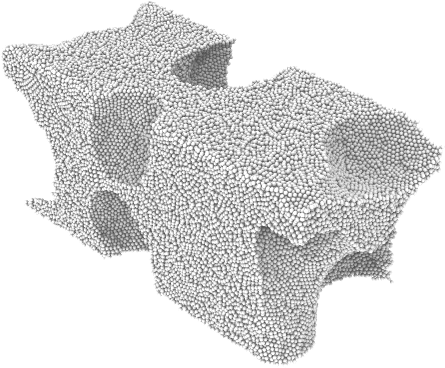
\includegraphics[width=0.40\textwidth]{./Figures/unstable}
  &
  \hspace{3mm}
  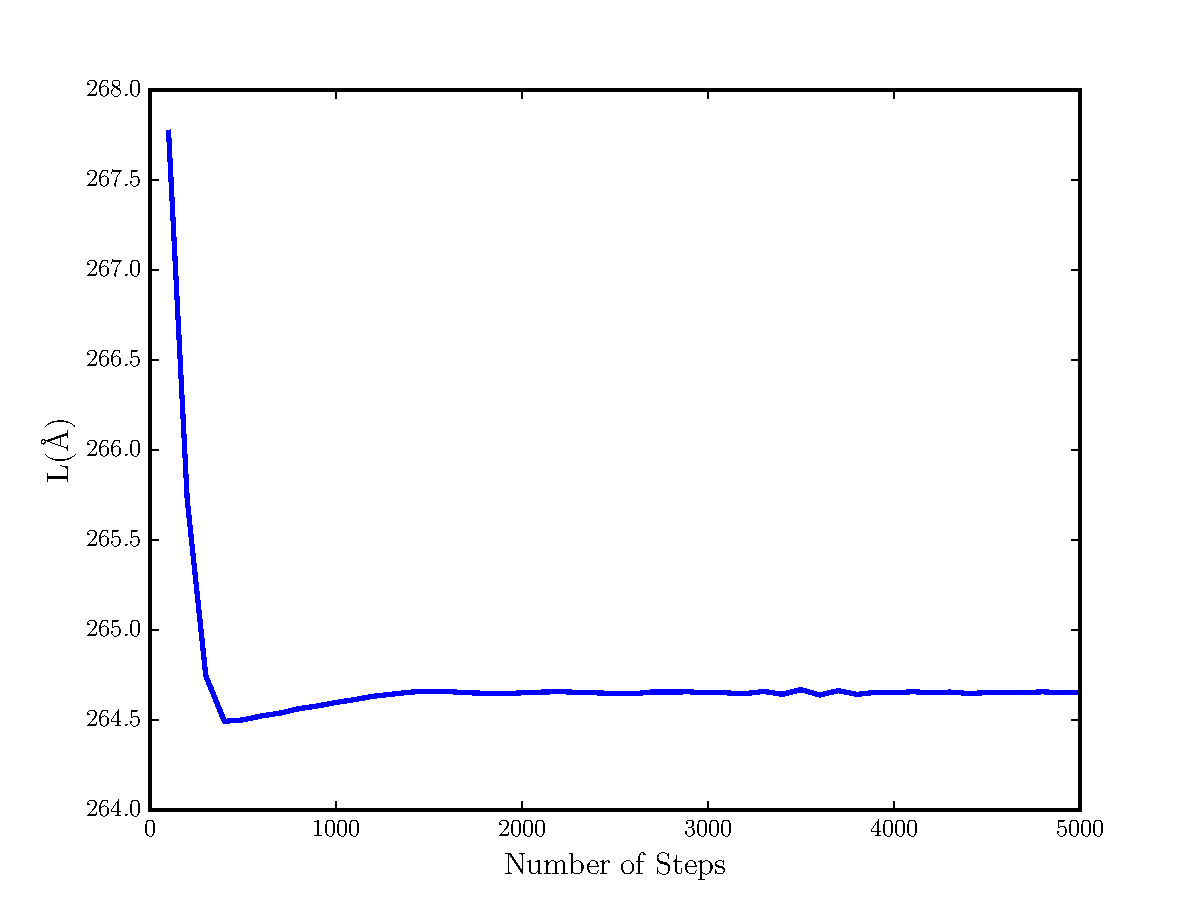
\includegraphics[width=0.50\textwidth]{./Figures/lx_npt}
  \\ (a) & (b)
  \end{tabular}
\caption{(a) A snapshot of the arrangement of atoms illustrating loss of
structural integrity of the Si bar. 
(b) Si bar length is plotted against the number of time steps during
the NPT ensemble stage of the simulation.}
\label{fig:dgsm1}
\end{center}
\end{figure}

To avoid this issue, we added an NPT ensemble prior to NVT in the NEMD simulation as shown in the
following diagram:

\begin{center}

NPT \hspace{5mm} $\rightarrow$ \hspace{5mm} NVT \hspace{5mm} $\rightarrow$ \hspace{5mm} NVE \hspace{5mm}
$\rightarrow$ \hspace{5mm} NVE
\\ \vspace{1mm}
\tiny [Relax the system]~[Equilibrate system to 300 K] \hspace{1mm} [Equilibrate thermostats] \hspace{4mm}
 [Generate Data]
\\ \vspace{1mm}

\tiny{N: Number of Atoms~~~P: Pressure~~~V: Volume~~~T: Temperature~~~E: Energy}
\end{center}

\noindent The NPT stage of the simulation was allowed to continue for a sufficiently long duration to ensure
that the system is relaxed to a steady value of the bar length as shown in Figure~\ref{fig:dgsm1}(b).

The following algorithm provides the sequence of steps that were used to obtain approximate estimates of the
sensitivity measures for the SW potential parameters. Note that the algorithm has been adapted to the 
specific application in this work. A generalized methodology with a more detailed discussion and its application
to different class of problems will be presented in~\cite{Vohra:2018}.

\bigskip

\begin{breakablealgorithm}
  \caption{Estimating parameter ranks using DGSM.}
  \begin{algorithmic}[1]
    \Procedure{DGSM}{}
      \State Generate $n_1$ points in $\mathbb{R}^{d}$.\Comment{$d$: 
             Number of parameters i.e. 7 in this case}
      \State Perturb each point along the $d$ directions to obtain a set of $n_1(d+1)$ points.
      \State Compute $\mu_i$ using model evaluations at the $n_1(d+1)$ points in Eq.~\ref{eq:mu}
      \State Determine initial ranks, $\mathcal{R}^{old}$ based on $\hat{\mathcal{C}_i\mu_i}$ values for $\theta_i$.
      \State set $k$ = 1\Comment{Iteration counter}
      \Do
        \State Generate $n_k$ new points in $\mathbb{R}^{d}$.
        \State Perturb each point along the $d$ directions to obtain a set of $n_k(d+1)$ points.
        \State Compute and store model evaluations at the $n_k(d+1)$ points.
        \State Compute $\mu_i$ using prior model evaluations at $(d+1)(n_1 + \sum_j^k n_j)$ points.
        \State Determine new ranks, $\mathcal{R}^{new}$ based on updated $\hat{\mathcal{C}_i\mu_i}$ values.
        \State Compute $max\_pdev$ = max$\left(\frac{|\mu_{i,k} - 
               \mu_{i,k-1}|}{ \mu_{i,k-1}}\right)$.\Comment{$max\_pdev$:
               Maximum percentage deviation in $\mu_i$ between successive iterations.}
        \State set $k$ = $k$ + 1
      \doWhile{($\mathcal{R}^{\tiny{new}}$ $\neq$ $\mathcal{R}^{\tiny{old}}$ {\bf or}  
               $max\_pdev$~$>~\tau$)\Comment{$\tau$:~Tolerance}}
    \EndProcedure
  \end{algorithmic}
\end{breakablealgorithm}

\bigskip

%\texttt{Algorithm}
%
%\begin{algorithm}[H]
%\SetAlgoLined
%%\nonl \scriptsize{\textsc{Part I: Parameter Screening}}
%%\nonl \textbf{\texttt{Algorithm}}\;
%\texttt{Generate $n_1$ points in $\mathbb{R}^{d}$}\;
%\texttt{Perturb each point along the $d$ directions to obtain a set of $n_1(d+1)$ points}
%\texttt{\color{blue} $\%$~$d$: Number of parameters in the SW potential i.e. 7}\;
%\texttt{Compute $\mu_i$ using model evaluations at the $n_1(d+1)$ points in Eq.~\ref{eq:mu}}\;
%\texttt{Determine initial ranks, $\mathcal{R}^{old}$ of the parameters based on $\hat{\mathcal{C}_i\mu_i}$ values}\;
%\texttt{set $k$ = 1}
%\texttt{\color{blue}$\%$~$k$:~Iteration counter}\;
%\Repeat{\texttt{($\mathcal{R}^{\tiny{new}}$ $\neq$ $\mathcal{R}^{\tiny{old}}$ $\&$ 
%$max\_pdev$~$>\tau$)~\color{blue}$\%$~$\tau$:~Tolerance}}{
%\texttt{Generate $n_k$ new points in $\mathbb{R}^{d}$}\;
%\texttt{Perturb each point along the $d$ directions to obtain a set of $n_k(d+1)$ points}\;
%\texttt{Compute and store model evaluations at the $n_k(d+1)$ points}\;
%\texttt{Compute $\mu_i$ using prior model evaluations at $(d+1)(n_1 + \sum_j^k n_j)$ points}\;
%\texttt{Determine new ranks, $\mathcal{R}^{new}$ based on updated $\hat{\mathcal{C}_i\mu_i}$ values}\;
%\texttt{Compute $max\_pdev$ = max($\frac{|\mu_{i,k} - \mu_{i,k-1}|}{ \mu_{i,k-1}}$)}
%\texttt{\color{blue}$\%$~$max\_pdev$: Maximum percentage deviation in $\mu_i$ between successive iterations.}\;
%\texttt{set $k$ = $k$ + 1}\;
%}
%\end{algorithm}

For the present application, we begin with $n_1$ = 10 samples in the 7D parameter space and add 5 points
at each iteration. Using a tolerance, $\tau$ = 0.05, the above algorithm took 4 iterations i.e. 25 points to 
provide approximate estimates for $\mu_i$. Since finite difference was used to estimate the derivatives in
Eq.~\ref{eq:mu}, it required 25(7+1) i.e. 200 MD runs. It must be noted that although the computational effort
pertaining to the estimation of DGSM can be substantial, it is nevertheless several orders of magnitude smaller
than directly estimating the Sobol\textquotesingle~indices as mentioned earlier. 
In Figure~\ref{fig:ub}, we plot $\hat{\mathcal{C}_i\mu_i}$ as obtained for the SW parameters at the 
end of 4 iterations. It appears that $\gamma$ is significantly more important than other parameters, whereas NEMD
predictions are relatively less sensitive to $B$ and $p$. Large sensitivity towards 
$\gamma$ and $\alpha$ (cut-off radius) is in fact expected since  these two parameters impact the lattice
constant and hence the mean free path associated with the bulk thermal conductivity directly. 

\begin{figure}[htbp]
 \begin{center}
  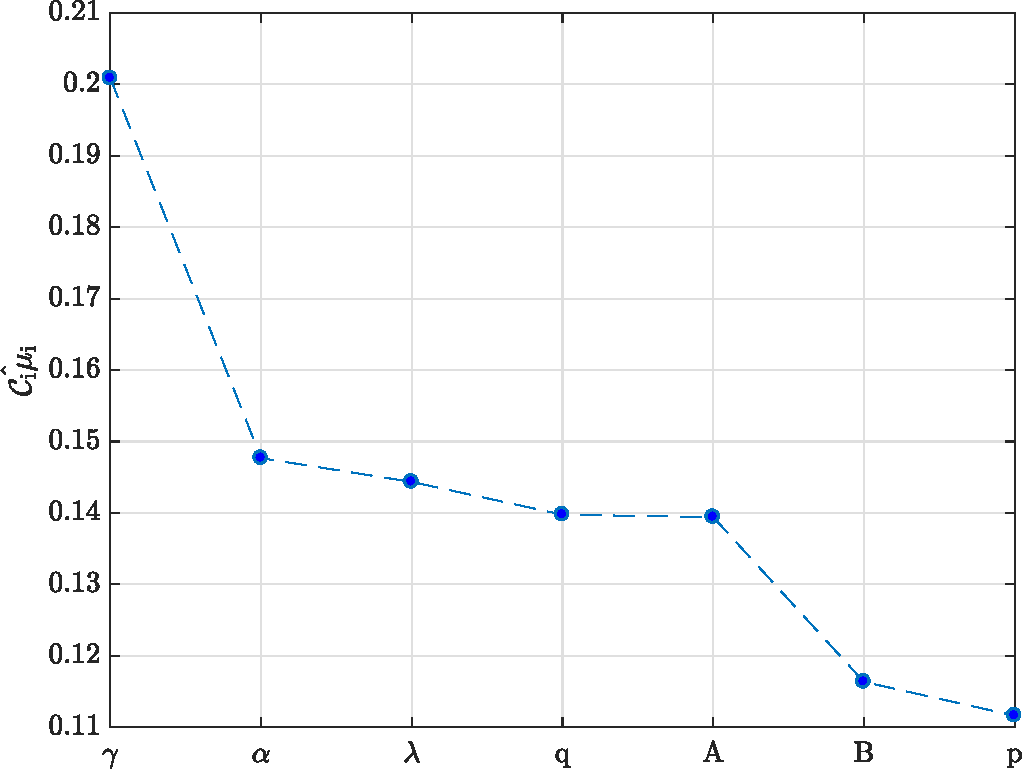
\includegraphics[width=0.65\textwidth]{./Figures/ub}
\caption{The quantity $\hat{\mathcal{C}_i\mu_i}$ as computed after 4 iterations and data at 200
points is plotted for each SW potential parameter.}
\label{fig:ub}
\end{center}
\end{figure}

In the following section, we exploit these observations based on DGSM to construct a reduced order surrogate.
The surrogate enables forward propagation of uncertainty in the SW potential to the bulk thermal conductivity 
estimates, and the estimation of Sobol\textquotesingle~sensitivity indices with minimal computational effort. 




























